\documentclass[final,hyperref={pdfpagelabels=false}]{beamer}

\usepackage{graphics, subfigure}
\usepackage{color}
\usepackage[portuguese]{babel}
\usepackage[utf8]{inputenc}
\usepackage[orientation=portrait,size=a0,scale=1.4]{beamerposter}
\usepackage{fp}% http://ctan.org/pkg/fp
\usepackage{wrapfig} % wrap text around figures
\usepackage{calc} % easy adding dimensions
\usepackage[export]{adjustbox} % left, right-align includegraphics
\usepackage{caption}
\usepackage{amsmath}
\newlength{\columnheight}
\setlength{\columnheight}{98cm}
\def\marginwidthratio{0.08}
\FPeval{\contentwidthratio}{1-\marginwidthratio}
\FPeval{\tightcontentwidthratio}{1-(\marginwidthratio / 2)}
\def\insidecolumnsinter{0.05}

\graphicspath{{figures/}}
\newlength{\insidecolumnwidth}%
\newlength{\intercolumnwidth}%
\newlength{\titleheight}%
% Colors %%%%%%%%%%%%%%%%%%%%%%%%%%%%%%%%%%%%%%%%%%%%%%%%%%%%%%%%%%%%%%%%%%%%%

\definecolor{green_butantan}{RGB}{0,112,60}
\definecolor{c_purple}{RGB}{56,3,52}
\definecolor{c_blue}{RGB}{41,68,107}
\definecolor{alert_blue}{RGB}{70, 130, 220}
\definecolor{c_green}{RGB}{87,184,9}
\definecolor{green2}{RGB}{76,196,93}
\definecolor{green3}{RGB}{76,173,138}
\definecolor{turquoise}{RGB}{39,94,102}
\definecolor{c_orange}{RGB}{255,149,28}
\setbeamertemplate{navigation symbols}{}  % no navigation on a poster
\setbeamercolor*{block title}{fg=green_butantan!80,bg=white}
\setbeamerfont{footline}{size=\large}
%\setbeamerfont{block title}{size=\large,series=\bf}
\setbeamerfont{block title}{size={\fontsize{64}{24}}, series=\bfseries}
\setbeamerfont{title}{size={\fontsize{83}{10}}}
\setbeamerfont{author font}{size={\fontsize{56}{10}}}
\setbeamerfont{supervisor font}{size={\fontsize{50}{10}}}


% Itemize %%%%%%%%%%%%%%%%%%%%%%%%%%%%%%%%%%%%%%%%%%%%%%%%%%%%%%%%%%%%%%%%%%%%
\setbeamertemplate{itemize item}{\color{green_butantan}{\textbf{$\bullet$}~}\color{black!50}}
\setbeamertemplate{itemize/enumerate body begin}{\color{black!80}}
\setbeamertemplate{itemize subitem}{\color{green_butantan}{\textbf{\diamond}~}}
\setbeamertemplate{caption}[numbered]
\setbeamercolor{caption}{fg=black!80}
\setbeamercolor{caption name}{fg=green2}
\setbeamercolor*{enumerate item}{fg=green_butantan}
\setbeamercolor*{enumerate subitem}{fg=green_butantan}
\setbeamercolor*{enumerate subsubitem}{fg=green_butantan}
\setbeamerfont{enumerate item}{series=\bf}
\setbeamercolor*{background canvas}{bg=white}



\newcommand{\leftcolumn}[1]{%
\begin{column}{.49\textwidth}%        
\begin{minipage}[T]{\textwidth}%
\parbox[t][\columnheight]{\textwidth}{#1}%
\end{minipage}%
\end{column}%
}
\newcommand{\rightcolumn}[1]{%
\begin{column}{.49\textwidth}%        
\begin{minipage}[T]{\textwidth}%
\parbox[t][\columnheight]{\textwidth}{#1}%
\end{minipage}%
\end{column}%
}

\newcommand{\customparagraph}[2]{%
\parbox[t][]{\contentwidthratio\textwidth}{%
%\hspace*{2cm}%
#2}%
\vspace*{#1}%
~\\%
}
\newcommand{\paragraph}[1]{%
\parbox[t][]{\contentwidthratio\textwidth}{%
%\hspace*{2cm}%
#1}%
\vspace*{2cm}%
~\\%
}

\newcommand{\tightparagraph}[1]{%
\vspace*{-.5cm}\parbox[t][]{\textwidth}{%
%\hspace*{2cm}%
#1}%
~\\%
}

\newcommand{\leftfigparagraph}[4]{%
\parbox[t][]{\contentwidthratio\textwidth}{%
\setlength\intextsep{0pt}%
\begin{wrapfigure}[#3]{L}{#2cm+1cm}%
\includegraphics[width=#2cm,left]{#1}%
\end{wrapfigure}%
%\hspace*{2cm}%
#4}%
\vspace*{2cm}%
~\\%
}

\newcommand{\rightfigparagraph}[4]{%
\parbox[t][]{\contentwidthratio\textwidth}{%
\setlength\intextsep{0pt}%
\begin{wrapfigure}[#3]{R}{#2cm+1cm}%
\includegraphics[width=#2cm,right]{#1}%
\end{wrapfigure}%
%\hspace*{2cm}%
#4}%
\vspace*{2cm}%
~\\%
}


\newcommand{\myimage}[2]{%
\scalebox{#2}{\includegraphics{#1}}%
~\\%
}

\newcommand{\mycenteredimage}[2]{%
\begin{center}%
\scalebox{#2}{\includegraphics{#1}}%
\end{center}%
}

\newcommand{\insidecolumns}[4]{%
\FPeval{\insidecolumnsnoncontent}{\marginwidthratio + \insidecolumnsinter}
\FPeval{\insidecolumnscontent}{1 - \insidecolumnsnoncontent}
\setlength{\insidecolumnwidth}{\insidecolumnscontent\textwidth}%
\setlength{\intercolumnwidth}{\marginwidthratio\textwidth}%
\vspace{-2cm}%
\begin{columns}[t,onlytextwidth]%
%\vrule{}%
\begin{column}{.5\intercolumnwidth}~\end{column}%
%\vrule{}%
\begin{column}{#1\insidecolumnwidth}%
\begin{flushleft}%
#3~%
\end{flushleft}%
\end{column}%
%\vrule{}%
\begin{column}{\insidecolumnsinter\textwidth}~\end{column}%
%\vrule{}%
\begin{column}{#2\insidecolumnwidth}%
\begin{flushright}%
#4~%
\end{flushright}%
\end{column}%
%\vrule{}%
\begin{column}{.5\intercolumnwidth}~\end{column}%
%\vrule{}%
\end{columns}%
\vspace*{2cm}%
}

\newcommand{\myitemize}[1]{%
\vspace*{-2cm}%
\hspace*{1cm}\parbox[t][]{0.9\textwidth}{%
\begin{itemize}%
#1%
\end{itemize}%
}%
\vspace*{3cm}%
}

\newcommand{\myenumerate}[1]{%
\vspace*{-2cm}%
\hspace*{1cm}\parbox[t][]{0.9\textwidth}{%
\begin{enumerate}%
#1%
\end{enumerate}%
}%
\vspace*{3cm}%
}

\newcommand{\mycite}[1]{{\color{c_green_dark}\textbf{$^{#1}$}}}

\setbeamertemplate{block begin}{%
  \begin{beamercolorbox}[ht=4cm,sep=1cm,leftskip=0.5cm]{block title}%
    \usebeamerfont*{block title}%
     \insertblocktitle\\%
     \noindent\makebox[\textwidth]{\hspace*{2cm}\color{c_green!60}\rule{0.95\textwidth}{5pt}\hspace{5cm}}%
  \end{beamercolorbox}%
  \usebeamerfont{block body}%
  \vspace*{.5cm}%
  \begin{beamercolorbox}[leftskip=1.5cm]{block body}%
  \color{black!80}
}

\setbeamertemplate{block end}{%
\end{beamercolorbox}%
% \vspace*{1cm}%
}

%%%%%%%%%%%%%%%%%%%%%%%%%%%%%%%%%%%%%%%%%%%%%%%%%%%%%%%%%%%%%%%%%%%%%%%%%%%%%%%%%%%%%%%%%
\setbeamertemplate{headline}{  
  \leavevmode

  \begin{beamercolorbox}[wd=\paperwidth]{headline}
      \vspace*{2cm}
    \begin{columns}[T]
      \begin{column}{.7\paperwidth}
      	\vspace*{1cm}
        \raggedleft
        \color{c_green}
        \textbf{\Large{\inserttitle}}\\[1ex]%
        \color{turquoise}
        \large{\insertauthor}\\[1ex]%
        \normalsize{\insertinstitute}\\[1ex]%
      \end{column}
      %\begin{column}{.01\paperwidth}
      %\end{column}
      \begin{column}{.25\paperwidth}
          
\includegraphics[width=.85\linewidth]{figures/institutions/butantanuspcetics3.png}
      \end{column}
      %\begin{column}{.03\paperwidth}
      %\end{column}
    \end{columns}
      \vspace*{1.5cm}
  	\setlength{\titleheight}{20pt}%
	
  \end{beamercolorbox}
  \vfill
}


%%%%%%%%%%%%%%%%%%%%%%%%%%%%%%%%%%%%%%%%%%%%%%%%%%%%%%%%%%%%%%%%%%%%%%%%%%%%%%%%%%%%%%%%%
\setbeamertemplate{footline}{
  \begin{beamercolorbox}[wd=\paperwidth]{upper separation line foot}
    \rule{0pt}{3pt}
  \end{beamercolorbox}
  \leavevmode%
  \begin{beamercolorbox}[ht=4ex,leftskip=2em,rightskip=2em]{author in head/foot}%
	\color{black}\phantom{a}
    \hfill
	\color{black}\{marcelo.reis, gustavo.matos \}@butantan.gov.br
    \vskip1ex
  \end{beamercolorbox}
  \vskip0pt%
  \begin{beamercolorbox}[wd=\paperwidth]{lower separation line foot}
    \rule{0pt}{3pt}
  \end{beamercolorbox}
}

\usepackage{mhchem}


%%%%%%%%%%%%%%%%%%%%%%%%%%%%%%%%%%%%%%%%%%%%%%%%%%%%%%%%%%%%%%%%%%%%%%%%
 
\title{\usebeamerfont*{title} Identification of cell signaling pathways 
    based on \\biochemical reaction kinetics repositories
}

\author{\vspace*{.5cm} \usebeamerfont*{author font} Gustavo Estrela de 
    Matos$^{\text{a, b, c}}$ \\ 
    \vspace*{.5cm}{\usebeamerfont*{supervisor font} Hugo
    A. Armelin$^{\text{b, c}}$, Marcelo S. Reis$^{\text{b, c}}$}}

\institute{%
    $^{\text{a}}$Institute of Mathematics and Statistics, University of
    São Paulo, Brazil\\%
$^{\text{b}}$Center of Toxins, Immune-response and Cell Signaling
(CeTICS), Instituto Butantan, Brazil\\%
$^{\text{c}}$Special Laboratory of Cell Cycle, Instituto Butantan,
Brazil}


\setbeamercolor{alerted text}{fg=alert_blue}

%%%%%%%%%%%%%%%%%%%%%%%%%%%%%%%%%%%%%%%%%%%%%%%%%%%%%%%%%%%%%%%%%%%%%%%%
\begin{document}


\renewcommand{\figurename}{Fig.}

\begin{frame}
\begin{columns}

\leftcolumn{ 
\begin{block}{Cell Signaling Pathways}%
\paragraph{
    Cell Signaling is a mechanism that allows the cell to change its 
    behaviour according to the environment.
\begin{figure}
    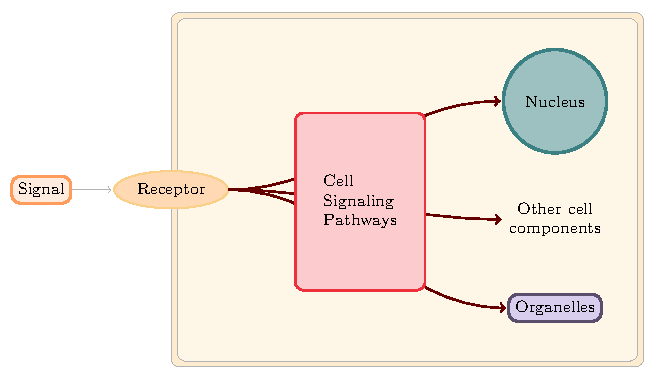
\includegraphics[width=.7\textwidth]{csp/signaling_mechanism.pdf}
\end{figure}
    A signal flows in a cell thorugh a cell signaling pathway, which can
    be characterized by a \alert{sequence of chemical reactions}.
}
\leftfigparagraph{csp/western_blot.png}{15}{6}{
    \hspace{1em}\\
    We can summarize the state of a cell signaling pathway by measuring
    the concentration over time of some chemical species that are
    present on the pathway, yielding experimental data D.
}
\end{block}

%%%%%%%%%%%%%%%%%%%%%%%%%%%%%%%%%%%%%%%%%%%%%%%%%%%%%%%%%%%%%%%%%%%%%%%%                                     
\begin{block}{Identification of Signaling Pathways}%
\paragraph{
    What is the structure of a cell signaling pathway, given a set of 
    concentration measurements? We answer this question
    with a computational model, created for \alert{a set of chemical
    reactions}, that can reproduce the concentration dynamics observed 
    experimentally. These models are created using the laws of mass 
    action, deriving a system of ordinary differential equations.
}
\paragraph{
    As an example, we can model the following equation:
    \begin{equation*}
        \ce{A + B -> C} \implies \frac{d[C]}{dt} = k[A][B]
    \end{equation*}
    Where $k$ is a reaction rate constant.
}
\paragraph{
    However, to derive the model, we still need to determine what is
    the set of chemical reactions of the signaling pathway.
}
\end{block}

%\vspace{-1cm}
%\begin{block}{Feature Selection}
%\paragraph{
    %We proposed to solve the identification of cell signaling pathways
    %as a feature selection problem. This problem consists of: given 
    %a set of features (reactions) and a score for each subset (the
    %\alert{quality of a model}), what is the best subset?
    %\begin{figure}
        %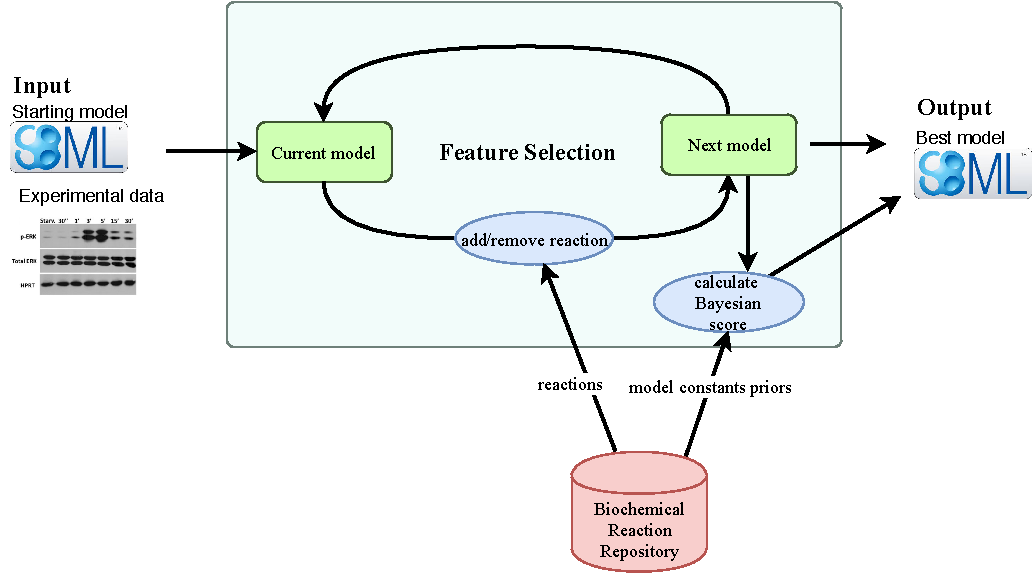
\includegraphics[width=\textwidth]{featsel/featsel.pdf}
    %\end{figure}
%}
%\end{block}


\begin{block}{Bayesian Ranking of Models}
    \paragraph{
    Given some experimental data $D$ and a model $M$ (composed by a
    \alert{a set o reactions}), we use an estimative of $p(D | M)$ as 
    a quality measure of model $M$. To create this estimative, we need
    to take samples from the posterior distribution of model parameters
    (reactions rate constants), denoted by $\theta | D, M$.
    %To determine the \alert{quality of a model} we implemented a 
    %score function that is an estimative of $p(D | M)$, which is the 
    %likelihood of observing experiment $D$ under the assumption that 
    %model $M$ is correct. To create this estimative we generate 
    %samples of the posterior distribution of model 
    %parameters ($\theta$).
    
    \begin{equation*}
        \underbrace{p (\theta | M, D)}_{\text{posterior}} \propto 
        \underbrace{p(D | M, \theta)}_{\text{likelihood}}
        \underbrace{p(\theta|M)}_{\text{prior}}
    \end{equation*}
}
    \leftfigparagraph{signetms_qr.png}{7}{4}{\hspace{1em}\\
        This ranking score was implemented as a Python package 
        called SigNetMS. This is an open source software and 
        it is available on GitHub: github.com/gustavoem/SigNetMS.
    }
\end{block}
%\vspace{-1cm}
\begin{block}{Acknowledgements}%
\vspace*{-0.5cm}%
\begin{figure}[h]
    \begin{tabular*}{0.7\textwidth}{c@{\extracolsep{\fill}}cc}
    \centering
    \subfigure {
        
\includegraphics[clip=true,
        width=0.2\textwidth]{institutions/FAPESP.jpg}
    }
    &
    %\subfigure {
        %
\includegraphics[clip=true,
        %width=0.2\textwidth]{institutions/FAPESP.jpg}
    %}
    &
    \subfigure {
        
\includegraphics[clip=true,
        width=0.2\textwidth]{institutions/ime.png}
    }
    \end{tabular*}   
\end{figure}
\vspace*{1.5cm}%
\end{block}%


} % end \leftcolumn



%%%%%%%%%%%%%%%%%%%%%%%%%%%%%%%%%%%%%%%%%%%%%%%%%%%%%%%%%%%%%%%%%%%%%%%%
\rightcolumn{              
\begin{block}{The Proposed Methodology}%
\paragraph{
    We proposed to solve the identification of cell signaling pathways
    as a feature selection problem. This problem consists of: given 
    a set of features (\alert{candidate reactions}) and a score for each
    subset (\alert{estimative of $p(D|M)$}), what is the best subset?
    \begin{figure}
        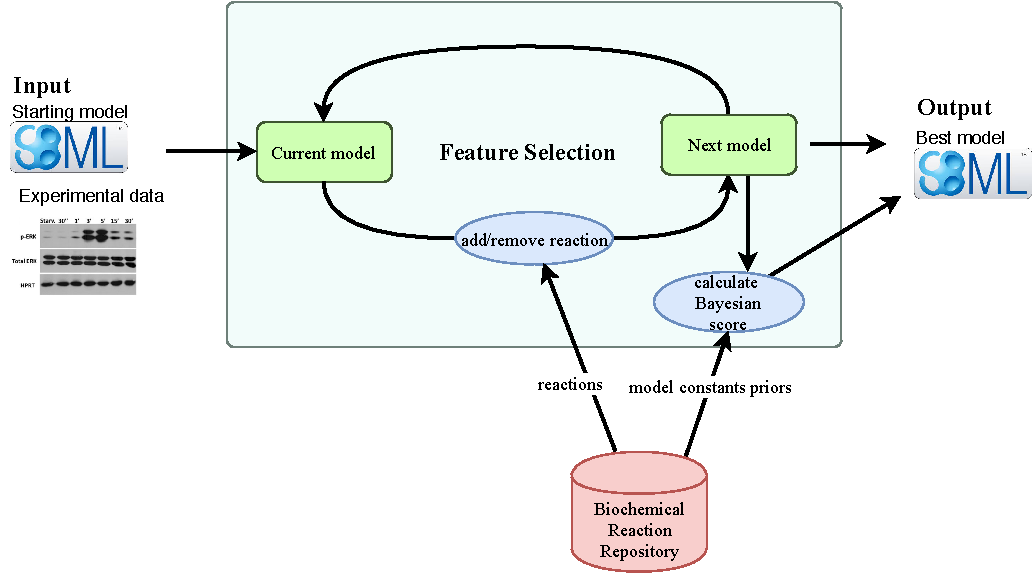
\includegraphics[width=.94\textwidth]{featsel/featsel.pdf}
    \end{figure}
    The set of candidate reactions is stored in a database, which also
    stores information about model parameters, namely, the reactions 
    rate constants. The information in the database is extracted from 
    other public databases.
}    
\end{block}

\vspace{-1em}
%%%%%%%%%%%%%%%%%%%%%%%%%%%%%%%%%%%%%%%%%%%%%%%%%%%%%%%%%%%%%%%%%%%
\begin{block}{Experiments}
\paragraph{
    We tested our ranking method on an experiment in which we create
    artificial experimental data and try to compare the found ranking 
    for four models.
\setcounter{subfigure}{0}
\begin{figure}[h]
    \centering
    \begin{tabular}{l r}
        \subfigure[Simulated model]{
        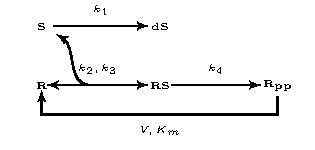
\includegraphics[clip=true,
        width=0.3\textwidth]{experiments/bioinformatics_model1.pdf}
    }
    &
    \subfigure[Simplified model]{
        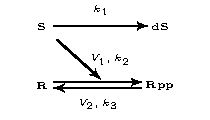
\includegraphics[clip=true,
        width=0.3\textwidth]{experiments/bioinformatics_model2.pdf}
    }
    \\
    \subfigure[Overly simplified model]{
        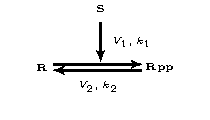
\includegraphics[clip=true,
        width=0.3\textwidth]{experiments/bioinformatics_model3.pdf}
    }
    &
    \subfigure[Model generalisation]{
        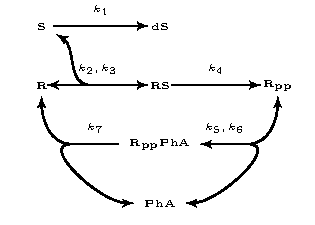
\includegraphics[clip=true,
        width=0.3\textwidth]{experiments/bioinformatics_model4.pdf}
    }

\end{tabular}
\end{figure}
    On this experiment we got the ranking: a $>$ b $>$ d $>$ c. This
    showed not only that we ranked the correct model first but also that 
    the complex models were penalized.
    
    {\color{c_green}\dotfill}
    \vspace{-.5em}

    \rightfigparagraph{experiments/surface_curve.png}{17}{7}{
    \hspace{1em} \\
    We also performed an experiment in which we add reactions
    iteratively to a model. We could have a glance of the surface of the 
    score metric over our search space. We could also notice that the 
    model error does not increase monotonically as we add more
    reactions.
}
}
\end{block}

\vspace{-2em}
\begin{block}{Conclusion and Future Work}
    In this work we were able to create a score metric that is able to
    rank models in a Bayesian approach and embed this function to a 
    feature selection procedure. The next tasks we aim to accomplish
    are:
    \begin{itemize}
        \item{Continue to study the surface of the search space;}
        \item{Apply the methodology in ERK signaling pathways of
            cell lines Y1 and HEK293.}
    \end{itemize}

\end{block}


%%%%%%%%%%%%%%%%%%%%%%%%%%%%%%%%%%%%%%%%%%%%%%%%%%%%%%%%%%%%%%%%%%%
\vspace*{.5cm}%
}% end of right column

\end{columns}
\end{frame}
\end{document}
